% siminos/reversal/recip1d.tex      pdflatex LC21; bibtex LC21
% temporary:  siminos/spatiotemp/chapter/LC21recip1d.tex
% $Author: hanliang $ $Date: 2021-12-24 16:09:56 -0500 (Fri, 24 Dec 2021) $

% Predrag 2021-08-08: shared with siminos/reversal/LC21.tex

\section{Reciprocal lattice}
\label{sect:LC21recip1d} % started with {sect:RhombCornerFT}

ChaosBook conventions:
\renewcommand{\cssp}{\ensuremath{\tilde{\phi}}}                % Complex state space point

$\omega = e^{2i\pi/\cl{}}$

$\cssp_k=x_k+i\,y_k = |\cssp_k| e^{i\theta_k}$

$q_k=2\pi{k}/\cl{}$,

$\cl{}$ is the Bravais cell period

\bigskip

Think of a solution of a discrete time dynamical system (iterations of a map) as a
1\dmn\ temporal {\lattstate} with the field on each site labeled by integer
time.
Were the lattice $d$\dmn, defined by Bravais cell vectors $\{\mathbf{a}\}$, a
crystallographer would immediately move to the \emph{reciprocal}
lattice,
\( %beq
\tilde{\lattice}_{\mathbf{b}} = \{k \mathbf{b}\,|\, k \in \mathbb{Z}\}
\,,
\) %ee{LC21:Rcpr1dLatt}
whith the {reciprocal}
lattice basis vectors $\{\mathbf{b}\}$ satisfing
\( %beq
\mathbf{b} \cdot \mathbf{a} = 2 \pi
\,.
\) %ee{LC21:Rcpr1dVect}
On the {reciprocal} lattice translations are
quotiented out, and calculations are restricted to a finite
{Brilluoin zone} (this is the {`Bloch theorem'} of
solid state physics). Here we work on a 1\dmn\ lattice with unit
lattice spacing 1, so the reciprocal lattice spacing is $2\pi/1=2\pi$, with
the (first) Brillouin zone from $k=-\pi$ to $k=\pi$.

A period-$\cl{}$ {\lattstate} lives on a discrete 1-torus (a ring or
necklace) of period-$\cl{}$, and if its law is time-invariant, its orbit, the set of
{\lattstate}s related to it by cyclic translations, are
physically equivalent. The symmetry is the cyclic group
\Cn{n}, and one only needs to count and distinguish \Cn{n} \emph{{\orbit}s},
compute only one {\lattstate} per each orbit.
The smart way to do this is by going to the irreducible representations
of \Cn{n} by the discrete Fourier transform.

In the $\cl{}$\dmn\ permutation representation,
the elements of the \Cn{n} are generated by
the $[\cl{}\!\times\!\cl{}]$ shift matrix
$\shift$ \refeq{hopMatrix} which
 translates for\-ward-in-time the {\lattstate} \refeq{1dLattStatC_n} by one site,
$\transp{(\shift \Xx)}=(\ssp_1,\ssp_1,\cdots,\ssp_{\cl{}-1},\ssp_0)$.
After $\cl{}$ shifts, the {\lattstate} returns to the initial
state, yielding the characteristic equation for the matrix $\shift$
\beq
\shift^\cl{}-\id=0
\,,
\ee{shift2n}
whose eigenvalues are $\cl{}$th roots of unity, and the $\cl{}$ complex
eigenvectors are also built from roots of unity
\bea
\{\lambda_k\} &=& \{1, \omega, \omega^2,\cdots, \omega^{\cl{}-1}\}
                \,,\quad
                  \omega=\e^{2\pi\mathrm{i}/\cl{}}
                \continue
\tilde{e}_k   &=&
    \frac{1}{\sqrt{\cl{}}}
    (1, \omega^k, \omega^{2k}, \ldots, \omega^{k(\cl{}-1)})
    \,,\qquad k=0, 1,\ldots, \cl{}-1
\,.
\label{FourierModes}
\eea
In the $\{\tilde{e}_k\}$ discrete Fourier basis,
the shift matrix is diagonal, $\shift_{jk}=\omega^k\,\delta_{jk}$,
and
an $\cl{}$\dmn\  $\cl{}$
{\lattstate} vector $\Xx$ is mapped onto a $\cl{}$\dmn\ {reciprocal}
lattice complex vector
\beq
(\cssp_{0},\cssp_{1},\cssp_{2},\dots,\cssp_{\cl{}-1})
=
(\cssp_{0},|\cssp_1|e^{i\theta_1},|\cssp_2|e^{i\theta_2},
     \dots,|\cssp_{\cl{}-1}|e^{i\theta_{\cl{}-1}})
\,.
\eeq
The dynamics is breathtakingly simple on the reciprocal lattice.
Spatial period-$\cl{}$
Bravais cell maps onto a regular $\cl{}$-gon in the reciprocal lattice.
repeats of shorter {\lattstate}s sit on the boundaries of the fundamental domain.
Lattice shift $\shift_j$ maps out the $\Group$-orbit by running on
circles, and orbits visit the $1/2\cl{}$ wedge only once, so the points
in the fundamental domain represent an orbit each.


with all reciprocal
lattice Brillioun zone solutions {\orbit}s in an $1/n$ sliver of a
$\cl{}$-gon.
If $\cl{}$ is prime, this is irreducible; if it is a multiple of a
prime, one should remove those solutions, as they have already been
accounted for.


The symmetry is
\Cn{n}, and one needs to distinguish \Cn{n} orbits
(''{prime cycle}s'' in ChaosBook; one per each orbit).
The right way to do this is by going to
\Cn{n} irreps, ie, by the discrete Fourier transform, with all reciprocal
lattice Brillioun zone solutions {\orbit}s in an $1/n$ sliver of a
$\cl{}$-gon. If $\cl{}$ is prime, this is irreducible; if it is a multiple of a
prime, one should remove those solutions, as they have already been
accounted for.

\bigskip

No self-respecting crystallographer would be drawing longer and longer
Bravais {\lattstate}s \refeq{reflSymOdd}-\refeq{reflSymEvens1} - they
eventually run off the sheet of paper, no matter how wide.
A professional crystallographer plots all {\lattstate}s snugly together
in the first Brillouin zone, where the translational orbit of a
{\lattstate} is -literally- a circle, symmetric  {\lattstate}s sit on
boundaries of point group's fundamental domain, and everything is
maximally diagonalized in term's of space group \Group\ irreps.

Consider
\[
\rho_{\vec{G}}(\vec{x})= e^{i\vec{G}\cdot\vec{r}(\vec{x})}
\,,
\]
where $\vec{G}$ is a reciprocal lattice vector. By definition,
$\vec{G}\cdot\vec{a}$ is an integer multiple of $2\pi$, $\rho_{\vec{G}}=1$ for
lattice vectors.
For any other state, reciprocal {\lattstate} is given by
\[
e^{i\vec{G}\cdot\vec{u}(\vec{x})} \neq 1
\,.
\]

When a
cube is a building block that tiles a $3D$ cubic lattice, it is referred
to as the `elementary' or `Wigner-Seitz' cell, and its Fourier transform
is called `the first Brillouin zone' in `the reciprocal space'.



%\item[2018-04-18 Predrag]
the time-reversal pairs
to be the complex-conjugate pairs in Fourier space, as \Cn{\infty} shift
moves them in opposite directions.

The eigenvectors of the translation operator which satisfy the
periodicity of the Bravais lattice % \refeq{2DBravLatt}
are plane waves of form:
\beq
f_\mathbf{k}(\mathbf{z}) = e^{i \mathbf{k} \cdot \mathbf{z}}
  \,, \quad
\mathbf{k} \in \overline{\lattice}
\,,
\ee{LC21:Rcpr1dEgnVect}
where the wave vector $\mathbf{k}$ is on the reciprocal lattice
$\overline{\lattice}$.

 A general plane wave does not
satisfy the periodicity, unless
\beq
e^{i {k} \cdot {R}} = 1
\, .
\ee{LC21:PrdicPlaneWave}
Since ${R}$ is a vector from the Bravais lattice $\lattice$, the wave
vector $\mathbf{k}$ must lie in the reciprocal lattice of $\lattice$:
\beq
\mathbf{k} \in \lattice^*
\,,\quad
\lattice^* =
\left\{ m \mathbf{b}\,|\,m \in \mathbb{Z}\right\} \, ,
\ee{LC21:RcprocalLattice}
where the primitive reciprocal lattice vectors $\mathbf{b}$ satisfies:
 \beq
\mathbf{b} \cdot \mathbf{a} = 2 \pi
\, .
\ee{LC21:RcprocalLattBasis}


% \item[2020-01-23 Predrag]
Barvinok \arXiv{/math/0504444}:
\\
Let $V$ be a $d$-dimensional real vector space with the scalar product
$\langle \cdot, \cdot \rangle$
and the corresponding Euclidean norm $\| \cdot\|$. Let $\lattice \subset V$ be a lattice
and let  $\lattice^{\ast} \subset V$ be the {\it dual} or the {\it reciprocal} lattice
\[
\lattice^{\ast}=\Bigl\{x \in V: \quad \langle x, y \rangle \in {\Bbb Z}
\quad
\mbox{ for all } \quad y \in \lattice \Bigr\}
\,.
\]

\subsection{Reciprocal {\lattstate}}

An infinite {\lattstate} is periodic if the state is invariant under the action of a translation group.
A translation group can be described by a Bravais lattice, the vector in
which determines the direction and distance of the translation. When the dynamical system
has time translation symmetry, the defining equation of the system is invariant under translations.
So it is natural to use the eigenvectors of the translation operator to study the {\lattstate}s of the
system.

The eigenvectors of translation operators are plane waves defined on the lattice. But to study
the {\lattstate}s, we need to require that the plane wave also satisfies the periodic
condition. Generally, a $d$\dmn\ Bravais lattice can be described by:
\bea
{\lattice} = \left\{\sum_{i=1}^d n_i \mathbf{b}_i | n_i \in \mathbb{Z}\right\}
\,,
\eea
where $\mathbf{b}_i$ is the $i$th primitive vector of the Bravais lattice.
And a plane wave on the $d$\dmn\ lattice is:
\bea
f_\mathbf{k}(\mathbf{z}) = e^{i \mathbf{k} \cdot \mathbf{z}}
\, ,
\eea
where $\mathbf{z}$ is the position of a lattice site, and $\mathbf{k}$ is the wave vector.
The periodicity given by the Bravais lattice $\lattice$ requires that:
\bea
f_\mathbf{k}(\mathbf{z}+\mathbf{R})
=f_\mathbf{k}(\mathbf{z})\,,
\quad
\mathbf{R} \in \lattice \,.
\eea
This condition can only be satisfied if the wave vector $\mathbf{k}$ exists on the
reciprocal lattice of the lattice $\lattice$:
\bea
\overline{\lattice} = \left\{ \sum_{j=i}^d n_i \mathbf{b}_i | n_i \in \mathbb{Z}\right\}
\,,
\eea
the basis vectors of which satisfy:
\bea
\mathbf{b}_i \cdot \mathbf{a}_j = 2 \pi \delta_{ij} \,.
\eea
Using these eigenvectors we can transform {\lattstate}s into reciprocal {\lattstate}s
by discrete Fourier transform.
Any {\lattstate} with the periodicity given by the Bravais lattice
$\lattice$ can be spanned by the plane waves with wave vectors in the
reciprocal lattice $\overline{\lattice}$. And since a {\lattstate} only has
values on lattice sites, we only need a finite number of plane waves to
span the {\lattstate}.
%For each {\lattstate} with periodicity given by a Bravais lattice,
%there exists a reciprocal {\lattstate}.


\subsection{Irreducible representations of the symmetry group}

\subsubsection{Cyclic groups}
\label{sect:LC21irrepsCn}

When we write period-$\cl{}$ {\lattstate}s as $\cl{}$\dmn\ vectors, and write the
shift operator $\shift$ as a $[\cl{} \times \cl{}]$ matrix \refeq{hopMatrix} which applies
cyclic permutation to the
{\lattstate}, the matrix representation of shift operators forms a permutation representation
of the cyclic translation group $\Cn{n}$. This permutation representation is a reducible
representation, i.e., it can be block diagonalized by a similarity transformation. Each block
on the diagonal is an irreducible representation (irrep).

The abelian group $\Cn{\cl{}}$ only has 1\dmn\ irreps. The permutation
representation of $\Cn{\cl{}}$ can be diagonalized by discrete Fourier transform. After the
transform the representation of the shift operator becomes,
\bea
\shift^{m}=
\left(
\begin{array}{ccccc}
1 \\
& \omega^m \\
& & \omega^{2m} \\
& & & \ddots \\
& & & & \omega^{(\cl{}-1)m}
\end{array}
\right) \,,
\quad
\omega=\e^{2\pi\mathrm{i}/\cl{}}
\,,
\eea
with {\lattstate}s projected onto 1\dmn\ subspaces
in which action of the shift operators is given by corresponding irrep.
As we transform the permutation representation of the shift operator into the block
diagonal form,
the {\lattstate}s
$(\ssp_{0},\ssp_{1},\ssp_{2},\dots,\ssp_{\cl{}-1})$
are spanned by the  Fourier modes basis,
with components
$(\cssp_{0},\cssp_{1},\cssp_{2},\dots,\cssp_{\cl{}-1})$.
When the shift operator acts on the {\lattstate}: $\Xx \to \shift \Xx$, the irreducible
representations act on the components in the corresponding subspace:
$\cssp_{k} \to \omega^k \cssp_{k}$.

As a concrete example, consider the temporal Bernoulli period-3 Bravais
lattice. It's a linear problem and all {\lattstate}s are easily computed
by hand. There is always the fixed point {\lattstate} $(0,0,0)$, and
for the stretching parameter value $s=2$, there are 6 {\lattstate}s
organized into 2 period-3 orbits, which we mark by a single {\lattstate}
per orbit, for example
$(\frac{1}{7},\frac{2}{7},\frac{4}{7})$
and
$(\frac{3}{7},\frac{6}{7},\frac{5}{7})$.
The remaining {\lattstate}s are their cyclic
permutations.

Discrete Fourier transform, \reffig{fig:HLBernoulliC3}, maps
these 7 {\lattstate}s into 7 reciprocal {\lattstate}s.
        \PC{2021-09-02} {
Why do you mark 1/8 in
\reffigs{fig:HLBernoulliC3}{fig:HLBernoulliC3InvariantOrbits}, when the
units are 1/7's? I see. You have $1/\sqrt{3}$ and $\pi$'s floating
around, unless you redefine units...
    }
The $k=1$ and $k=3-1$ wave-numbers reciprocal {\lattstate}s are complex
conjugates of each other because the {\lattstate}s are real.

Consider next the action of the shift operator $\shift$ on the reciprocal
{\lattstate}s.
In the $k=0$ subspace, the eigenvalue of any shift is 1, so the $k=0$
component of any reciprocal {\lattstate} is invariant under the shift.
In the $k=1$ and $k=2$ subspaces, the shift $\shift$ acts by complex
phase rotations $\exp(2 \pi \mathrm{i}/3)$ and $\exp(4 \pi
\mathrm{i}/3)$, with the two subspaces rotating counter clockwise and
clockwise by $2\pi/3$ in the complex plane: reciprocal {\lattstate}s that
belong to the same orbit lie on a circle in the complex plane, related by
complex rotations.
\refFig{fig:HLBernoulliC3} illustrates this; the two
orbits, built from reciprocal {\lattstate}s that are related by shifts,
are connected by blue lines.


%%%%%%%%%%%%%%%%%%%%%%%%%%%%%%%%%%%%%%%%%%%%%%%%%%%
\begin{figure}
  \centering
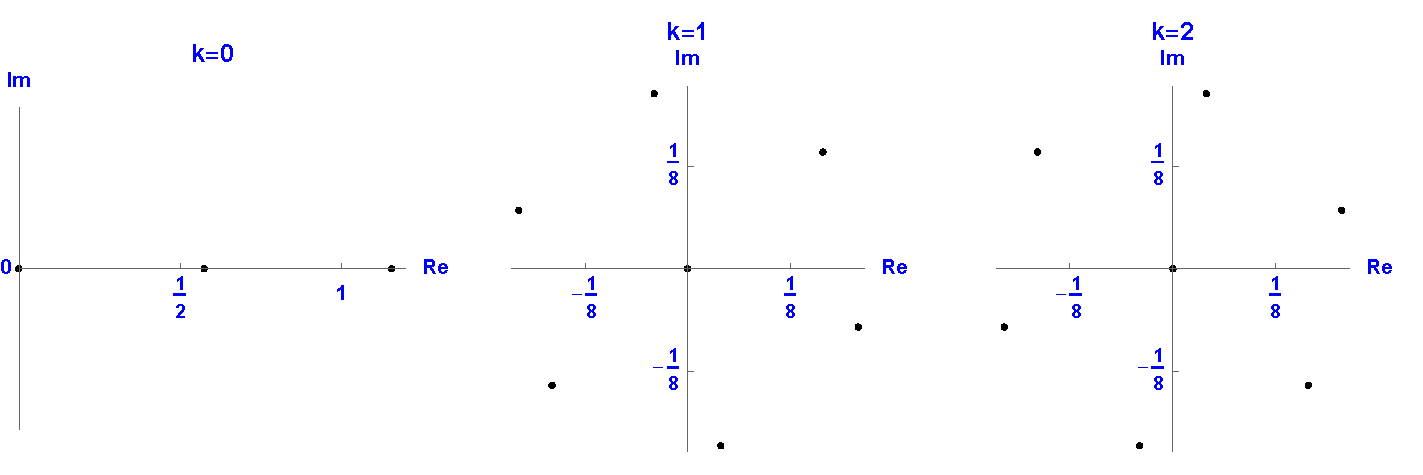
\includegraphics[width=\textwidth]{HLBernoulliC3}
  \caption{\label{fig:HLBernoulliC3}
Period-3 {\lattstate}s of the {temporal Bernoulli} with $s=2$, plotted in the $\Cn{3}$
permutation irreps subspaces. The components $\cssp_1$ and $\cssp_2$ are 
complex numbers in general. In the subspaces of $\cssp_1$ and $\cssp_2$,
the 2 triangles are 2 \Cn{3} orbits, and the state in the center is the fixed point.
}
\end{figure}
%%%%%%%%%%%%%%%%%%%%%%%%%%%%%%%%%%%%%%%%%%%%%%%%%%%

\subsubsection{Dihedral group}
\label{sect:LC21irrepsDn}

In the $\cl{}$\dmn\ space of the period-$\cl{}$ {\lattstate}s, the permutation representation
of the Dihedral group \Dn{\cl{}} can be generated by the shift operator matrix representation
\refeq{hopMatrix} and the reflection operator matrix representation:
\bea
\Refl=
\left(
\begin{array}{ccccc}
 1 &&&&0\\
  &  &  & 0 & 1 \\
  &  & \reflectbox{$\ddots$} & 1 &  \\
  & 0 & \reflectbox{$\ddots$} &  &  \\
  0& 1 &  &  &  \\
\end{array}
\right) \,.
\eea

The Dihedral group $\Dn{\cl{}}$ has: 2 1\dmn\ irreps and $[(\cl{}-1)/2]$
2\dmn\ irreps if $\cl{}$ is odd,
or 4 1\dmn\ irreps and $(\cl{}/2-1)$ 2\dmn\ irreps if $\cl{}$ is even.
If $\cl{}$ is odd, the permutation representation can be block diagonalized into irreps:
$A_0 \oplus E_1 \oplus \dots \oplus E_{(\cl{}-1)/2}$.
If $\cl{}$ is even, the permutation representation can be block diagonalized into irreps:
$A_0 \oplus B_1 \oplus E_1 \oplus \dots \oplus E_{\cl{}/2-1}$.

%%%%%%%%%%%%%%%%%%%%%%%%%%%%%%%%%%%%%%%%%%%%%%%%%%%
\begin{figure}
  \centering
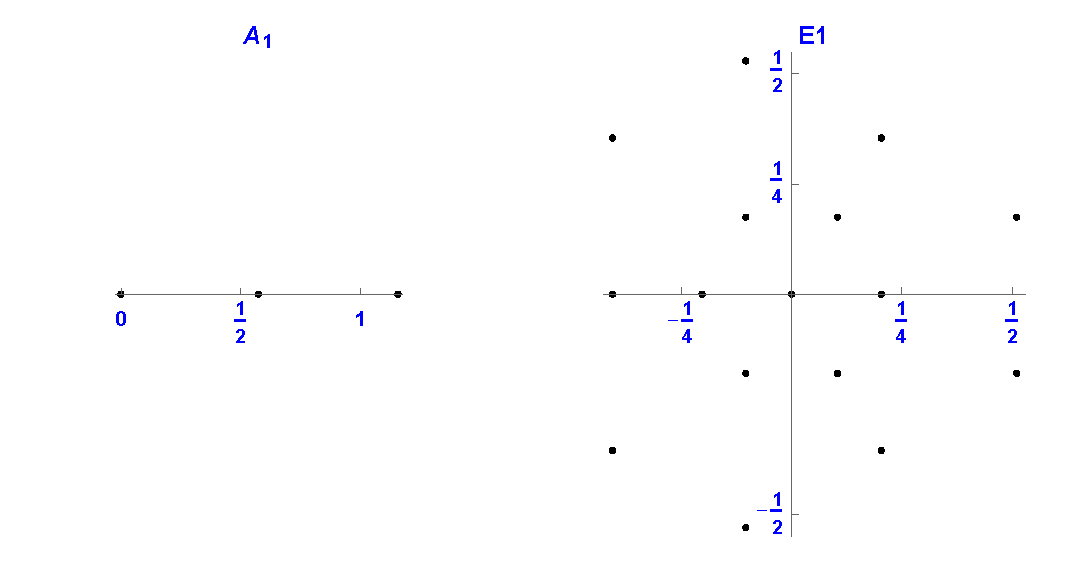
\includegraphics[width=0.8\textwidth]{HLCatmapD3}
  \caption{\label{fig:HLCatmapD3}
Period-3 {\lattstate}s of the $s=3$ \templatt, plotted in the $\Dn{3}$
permutation irreps subspaces $A_0+E$. In contrast with the
\Cn{\cl{}} complex irreps (see the \Cn{3} example
\reffig{fig:HLBernoulliC3}), the 2\dmn\ irrep $E\in\reals^2$ is real.
In the subspace of the $E$ irrep, 
{\lattstate}s that are related by cyclic permutations are connected by blue lines.
The 2 big triangles are a single \Dn{3} 6-{\lattstate}s orbit, what for
\Cn{3} is a pair of 3-{\lattstate}s orbits without time reversal symmetry.
The remaining 3 smaller triangles are 3 time-reversal symmetric orbits;
the pair in the middle is presumably related by the
 $\Dn{1}: S\ssp_i = 1-\ssp_i$ invariance specific to
the \templatt, a symmetry not yet taken into account. The state in
the center is the fixed point.
Red dashed lines are the reflection axes of the $\Dn{3}$ group. There are 4 states
on each reflection axis.
}
\end{figure}
%%%%%%%%%%%%%%%%%%%%%%%%%%%%%%%%%%%%%%%%%%%%%%%%%%%

When we use the similarity transformation to diagonalize the permutation representation,
the {\lattstate}s are transformed into the subspaces of the irreps.
The example of period-3 {\lattstate}s of \templatt\ with $s=3$ is shown in
\reffig{fig:HLCatmapD3}. The permutation
representation is block diagonalized by basis vectors: $e_0=1/\sqrt{3}(1,1,1)$,
$e_1=\sqrt{2/3}(\cos(2\pi/3),\cos(4\pi/3),1)$ and $e_2=\sqrt{2/3}(\sin(2\pi/3),\sin(4\pi/3),0)$.
The basis vector $e_0$ spans the subspace of the 1\dmn\ irrep $A_0$.
Basis vectors $e_1$ and $e_2$ span the subspace of the 2\dmn\ irrep $E$.

Period-3 {\lattstate}s of cat map with $s=3$ are mapped into the subspace
of the irreps $A_0$ and $E$ in \reffig{fig:HLCatmapD3}.
The irrep $A_0$ is the symmetric 1\dmn\ irrep, so in the subspace of $A_0$ the components
of {\lattstate}s are invariant under the action of the $\Dn{3}$ group.
In the 2\dmn\ subspace of the irrep $E$, the shift operator $\shift$ rotates the
{\lattstate}s clockwise by $2\pi/3$, while the reflection operator $\Refl$ reflects the {\lattstate}s
over the axis passing through the origin and pointing toward $(\cos(2\pi/3),\sin(2\pi/3))$.
In \reffig{fig:HLCatmapD3}
{\lattstate}s that are related by shifts are connected by blue lines.
The red dashed lines are reflection axis of the reflection operators.
The 2 big triangles in \reffig{fig:HLCatmapD3} subspace of $E$ are lattice states
that belong to 2 orbits which are related by time reflection. The rest 3 triangles
are lattice states from 3 orbits which are invariant under time reflection.

\subsection{Fundamental domain} % of the {\lattstate}}

Given the space of the field configuration and the symmetry group acting on it,
we can find a fundamental domain such that each orbit in this space
visits the fundamental domain only once.
Each {\lattstate} in the fundamental domain is a representative {\lattstate} of an
orbit.
    \PC{2021-10-12}{
    Please read our draft\rf{LC21}, and either follow
    our definition \refeq{1dLattStat} of {\em {\lattstate}},
    or replace it with some other definition.
    }

One method to find the fundamental domain is based on the decomposition
of the space into the subspaces of the irreps of the symmetry group.
A natural way to choose the fundamental domain is to divide in the
subspace of an irrep, where the irrep divides the subspace into the number
of copies that is equal to the order of the symmetry group.

For example, in the space of the field configuration with \Cn{\cl{}} symmetry, the $k=1$ subspace
spanned by the eigenstate $\tilde{e}_1$, defined in \refeq{FourierModes}, can be divided
into $\cl{}$ copies. One can choose the region in the complex plane of $k=1$ subspace
with argument $0\leq\arg(\cssp_{1})<2\pi/\cl{}$ to be the fundamental domain.
Each orbit can visit the fundamental domain only once. As shown in \reffig{fig:HLBernoulliC3},
there are 3 points in this region, which are representative {\lattstate}s of two different
period-3 orbits and the fixed point $0$.

If the space of the field configuration has \Dn{\cl{}} symmetry,
the subspace of the 2\dmn\ irrep $E_1$ can be divided
into $2\cl{}$ copies by the irrep. One can choose the fundamental domain to be the region
with polar angle between 0 and $\pi/\cl{}$, assuming that the horizontal axis is one of the
reflection axis of the irrep $E_1$. Each orbit only appears once in the fundamental domain,
as shown in \reffig{fig:HLCatmapD3}. Note that the two orbits related by
the time reflection are considered one orbit of the dihedral group.

What happens when {\lattstate}s appear on the boundary of the fundamental domain?
There are two possible situations. The first situation is that the {\lattstate} belongs to an
orbit with multiplicity less than the order of the symmetry group. For example,
in \reffig{fig:HLCatmapD3} subspace of $E$, there are 3 points in the fundamental domain
with polar angle equal to 0 or $\pi/3$. These 3 points are representative {\lattstate}s of orbits
with time reflection symmetry. The multiplicities of these orbits are 3 instead of 6.

The second situation is that the multiplicity of
the orbit of the {\lattstate} is equal to the order of the symmetry group
but the component in the subspace is 0. For example,
\[
\Xx = \frac{1}{104} (17, 51, 49, 43, 25, 75)
\]
is a period-6 {\lattstate} of the temporal Bernoulli
\refeq{LC21:1dBernLatt} with $s=3$. Using the discrete Fourier transform
this {\lattstate} becomes:
\[
\cssp =
\left(\frac{5}{2 \sqrt{6}},0,\frac{-5-3 i \sqrt{3}}{13
   \sqrt{6}},-\frac{\sqrt{3}}{4\sqrt{2}},\frac{-5+3 i \sqrt{3}}{13 \sqrt{6}},0\right) \,.
\]
This is a period-6 {\lattstate}. It belongs to an orbit that
contains 6 different {\lattstate}s. The $k=1$ component of this lattice
state is 0, which is on the boundary of the fundamental domain. To put this kind of
{\lattstate}s into the fundamental domain one needs to divide other subspaces.
For this lattice state the $k=2$ and $k=3$ components are not 0. The irreps divide
the $k=2$ subspace into 3 copies and the $k=3$ subspace into 2 copies. One way to
choose the fundamental domain in these subspaces is: the argument of the component
in the $k=1$ subspace is $0\leq\arg(\cssp_{1})<\pi/3$; if the $k=1$ component
is 0, the arguments of the components
in the $k=2$ and $k=3$ subspaces are $0\leq\arg(\cssp_{2})<2\pi/3{}$ and
$0\leq\arg(\cssp_{3})<\pi$. Each orbit is guaranteed to visit this fundamental
domain exactly once.

\bigskip
------------------------------------

If, in addition, the law is time-reversal (or time-inversion) invariant,
the symmetry includes time-reflection, ie, it is dihedral group \Dn{n}
with 2$\cl{}$ elements, so the reciprocal lattice should be a half of the
above 1/$\cl{}$ sliver of a $\cl{}$-gon, and irreps are now either 1 or 2
dimensional. Even $\cl{}$ is different from odd $\cl{}$, and solutions either appear
in pairs, or are self dual under reflection in 3 different ways.

Due to the time
reversal, all $k={2\pi}/{5}$ irrep states are the same as the
$k={4\pi}/{5}$ irrep states.
